%----------------------------------------------------------------------------------------
%	METODE
%----------------------------------------------------------------------------------------
\section*{METODE PENELITIAN}

Penelitian yang dilakukan terbagi menjadi beberapa tahapan proses. Gambar \ref{fig:tahapan} menunjukan tahapan proses tersebut.

\begin{figure}[h!] % Gunakan \begin{figure*} untuk memasukkan Gambar
\centering
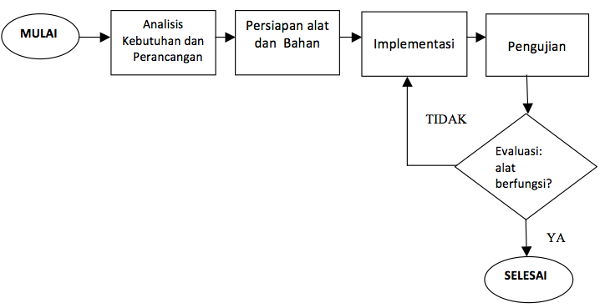
\includegraphics[width=200pt]{kolokium_contoh_gb1.png}
\caption{Tahapan proses penelitian}
\label{fig:tahapan}
\end{figure}

\subsection*{Analisa Kebutuhan dan Perancangan}

Tahapan ini menentukan komponen yang akan diperlukan dalam pembuatan alat. Komponen utama yang akan digunakan pada penelitian adalah mikrokontroler Arduino Uno, sedangkan komponen lain sebagai pendukung diantaranya kabel, resistor, speaker, LCD, \textit{keypad}, dan sebagainya. Arduino Uno digunakan karena mempunyai berbagai fungsi yang sudah terintegrasi di dalam satu modul mikrokontroler dan sudah siap pakai (arduino.cc). Mikrokontroller Arduino Uno dapat dilihat pada Gambar \ref{fig:uno}. Perancangan alat dilakukan setelah analisa kebutuhan terpenuhi. Gambar \ref{fig:alat} merupakan ilustrasi dari alat pengusir tikus yang akan dibuat.

\begin{figure}[h!]\centering % Gunakan \begin{figure*} untuk memasukkan Gambar
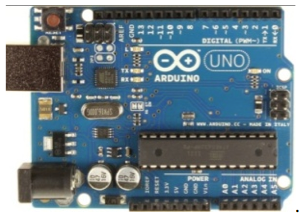
\includegraphics[width=150pt]{kolokium_contoh_gb2.png}
\caption{Arduino Uno}
\label{fig:uno}
\end{figure}

\begin{figure}[h!]\centering % Gunakan \begin{figure*} untuk memasukkan Gambar
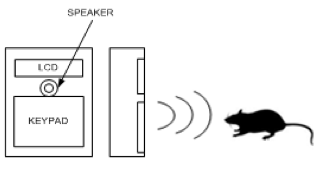
\includegraphics[width=200pt]{kolokium_contoh_gb3.png}
\caption{Ilustrasi alat}
\label{fig:alat}
\end{figure}

\subsection*{Persiapan Alat dan Bahan}

Kegiatan yang dilakukan pada tahap ini adalah mengumpulkan alat dan bahan yang akan digunakan pada penelitian. Persiapan dibagi menjadi 2, yaitu persiapan alat dan bahan untuk pembuatan alat dan persiapan alat dan bahan untuk pengujian alat. Persiapan pertama adalah mengumpulkan komponen yang akan digunakan dalam pembuatan alat seperti mikrokontroler Arduino Uno beserta komponen pendukung lainnya. Persiapan kedua adalah mengumpulkan alat dan bahan untuk pengujian seperti tikus, kandang tikus, alat perekam video dan lain-lain.

\subsection*{Implementasi}

Tahapan ini adalah melakukan implementasi dengan alat dan bahan yang telah dipersiapkan sebelumnya. Alat yang telah dirangkai kemudian diprogram agar dapat membangkitkan gelombang ultrasonik. Frekuensi yang akan dihasilkan oleh alat adalah antara 31-105 kHz. Nilai jangkauan tersebut sama dengan penelitian yang dilakukan oleh \citeauthor{SIMEON2013} (\cite*{SIMEON2013}). Gelombang ultrasonik yang keluar sesuai dengan input yang dimasukkan secara manual melalui \textit{keypad} dan nilai frekuensinya dapat dilihat pada LCD.

\subsection*{Pengujian}

Pengujian dibagi menjadi 2, yaitu pengujian frekuensi dan pengujian fungsi alat. Pengujian frekuensi dilakukan untuk menguji efisiensi frekuensi yang keluar dari alat dengan rumus:

\begin{equation}
\Phi = \frac{f_0}{f}\times 100\% \times \int_0^1x
\label{eq:persamaan}
\end{equation}

Berdasarkan persamaan \ref{eq:persamaan}

\noindent dengan $\Phi$ adalah efisiensi, $f_0$ adalah frekuensi yang dihasilkan, dan $f$ adalah frekuensi yang diinginkan.

Nilai frekuensi yang dibangkitkan oleh alat dicek melalui osiloskop. Pengujian kedua adalah pengujian fungsi alat terhadap tikus. Tikus yang digunakan sebagai objek percobaan adalah tikus putih dan tikus rumah yang berada di wilayah Kota Bogor. Tempat yang dijadikan sebagai tempat pengujian adalah 2 kandang yang dihubungkan oleh saluran penghubung yang dapat dilalui oleh tikus. Tikus dibiarkan beradaptasi dengan kandang sebelum pengujian alat dilakukan. Ilustrasi pengujian fungsi alat dapat dilihat pada Gambar \ref{fig:pengujian}.

\begin{figure}[h!]\centering % Gunakan \begin{figure*} untuk memasukkan Gambar
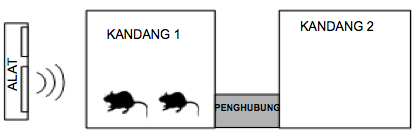
\includegraphics[width=200pt]{kolokium_contoh_gb4.png}
\caption{Ilustrasi pengujian alat}
\label{fig:pengujian}
\end{figure}

Jumlah tikus yang dimasukkan ke dalam kandang adalah 2 ekor dengan jenis kelamin yang berbeda. Pengamatan dilakukan dengan cara merekam tingkah laku tikus dengan alat perekam video yang telah dipasang pada kandang. Parameter yang digunakan pada pengujian ini adalah tingkat frekuensi yang efektif mempengaruhi tikus, jarak alat dan tikus yang optimum dan waktu yang diperlukan untuk mengusir tikus.

\subsection*{Evaluasi}
Pengujian yang dilakukan di tahap sebelumnya dievaluasi pada tahap ini. Pengujian pertama dinyatakan berhasil jika efisiensi frekuensi mencapai 100$\%$ artinya frekuensi yang dihasilkan sesuai dengan input yang dimasukkan. Pengujian kedua dinyatakan berhasil jika tikus yang berada pada kandang berpindah tempat ke kandang lain setelah terkena gelombang ultrasonik dari alat. Pengulangan implementasi dilakukan jika salah satu atau kedua pengujian dinyatakan tidak berhasil atau gagal.

\subsection*{Jadwal Kegiatan}
Penelitian ini akan dilakukan selama 4.5 bulan dengan rincian kegiatan seperti tercantum pada Tabel \ref{tab:jadwal}.
\begin{table*}[t!]
	\begin{center}
		\caption{Rencana Jadwal Penelitian}
		\label{tab:jadwal}
		\footnotesize
		\begin{tabular}{|l|c|c|c|c|c|c|c|c|c|c|c|c|c|c|c|c|c|c|}
			\hline
			\multirow{2}{*}{Kegiatan}&\multicolumn{2}{c|}{1}&\multicolumn{4}{c|}{2}&\multicolumn{4}{c|}{3}&\multicolumn{4}{c|}{4}&\multicolumn{4}{c|}{5}\\
			\cline{2-19}
			&3&4&1&2&3&4&1&2&3&4&1&2&3&4&1&2&3&4\\
			\hline
			Penyusunan Proposal Skripsi&\cellcolor{black}&\cellcolor{black}&\cellcolor{black}&\cellcolor{black}&&&&&&&&&&&&&&\\
			\hline
			Kolokium&&&&&\cellcolor{black}&&&&&&&&&&&&&\\
			\hline
			Perbaikan proposal&&&&&&\cellcolor{black}&&&&&&&&&&&&\\
			\hline
			Pengambilan data lapangan&&&&&&\cellcolor{black}&\cellcolor{black}&\cellcolor{black}&&&&&&&&&&\\
			\hline
			Pengolahan dan analisis data&&&&&&&&\cellcolor{black}&\cellcolor{black}&\cellcolor{black}&\cellcolor{black}&&&&&&&\\
			\hline
			Penulisan draft skripsi&&&&&&&&&&&&\cellcolor{black}&\cellcolor{black}&\cellcolor{black}&\cellcolor{black}&&&\\
			\hline
			Uji petik&&&&&&&&&&&&&&&&\cellcolor{black}&&\\
			\hline
			Sidang skripsi&&&&&&&&&&&&&&&&&\cellcolor{black}&\\
			\hline
			Perbaikan laporan penelitian&&&&&&&&&&&&&&&&&&\cellcolor{black}\\
			\hline
		\end{tabular}
		\normalsize
	\end{center}
\end{table*}


\subsection*{Contoh Penulisan}

Bagian ini sengaja diisi dengan beberapa contoh penulisan dalam LaTex untuk memudahkan menulis makalah dengan cepat menggunakan LaTex. Berikut adalah contoh membuat tabel yang dapat dirujuk. Misalnya, Tabel \ref{tab:daftarsaya} menjelaskan sesuatu yang terkait dengan naskah ini.

\begin{table}[hbt]
\caption{Daftar Nilai}
\centering
\begin{tabular}{llr}
\toprule
\multicolumn{2}{c}{Name} \\
\cmidrule(r){1-2}
First name & Last Name & Grade \\
\midrule
John & Doe & $7.5$ \\
Richard & Miles & $2$ \\
\bottomrule
\end{tabular}
\label{tab:daftarsaya}
\end{table}

Kadangkala kita juga perlu menuliskan suatu formula matematika dalam sebuah kalimat. Misalnya, ada formula matematika $\cos^3 \theta =\frac{1}{4}\cos\theta+\frac{3}{4}\cos 3\theta$, dimana penulisan formula ini berbeda dengan formula sebelumnya yang diberi referensi atau nomor formula yang dapat diacu di dalam sebuah teks kalimat.

Tabel \ref{tab:tag} menunjukkan contoh suatu tabel yang memiliki lebar melebihi kolom yang diinginkan, sehingga perlu diatur lebar sesuai yang diinginkan. Dalam hal ini digunakan paket \textit{tabulary}.

\begin{table}[h!]
\footnotesize
\caption{Deskripsi dokumen XML tanaman obat}
\centering
\begin{tabulary}{0.45\textwidth}{LL}
\toprule
\parbox{12em}{Nama Tag} & Deskripsi \\
\midrule
$<$dok$>$&Mewakili keseluruhan dokumen\\
$<$id$>$&Menjelaskan id dokumen\\
$<$nama$>$&Nama tanaman obat\\
$<$namal$>$&Nama latin tanaman obat\\
$<$deskripsi$>$&Deskripsi tanaman obat yang terdiri dari manfaat, habitus, bagian yang digunakan dan kandungan zat kimia\\
$<$fam$>$&Famili tanaman obat\\
$<$penyakit$>$&Penyakit yang dapat disembuhkan oleh tanaman obat.\\
\bottomrule
\end{tabulary}
\label{tab:tag}
\end{table}

\subsection*{Contoh Penulisan Algoritme}
Algoritme \ref{algo:max} dibuat untuk mendapatkan bilangan terbesar dari kumpulan bilangan yang terhingga.

\begin{algorithm}
\DontPrintSemicolon % Some LaTeX compilers require you to use \dontprintsemicolon instead
\KwIn{Himpunan $A=\{a_1, a_2, \ldots, a_n\}$}
\KwOut{Bilangan terbesar}
$max \gets a_1$\;
\For{$i \gets 2$ \textbf{to} $n$} {
  \If{$a_i > max$} {
    $max \gets a_i$\;
  }
}
\Return{$max$}\;
\caption{{\sc Max} mendapatkan bilangan terbesar}
\label{algo:max}
\end{algorithm}
